\documentclass[conference]{IEEEtran}

\IEEEoverridecommandlockouts
% The preceding line is only needed to identify funding in the first footnote. If that is unneeded, please comment it out.
\usepackage{cite}
\usepackage{float}
\usepackage{tabularx}
\usepackage{makecell}
\usepackage{multirow}
\usepackage{hhline}
\usepackage{amsmath,amssymb,amsfonts}
\usepackage{algorithmic,algorithm}
\usepackage{graphicx}
\usepackage{textcomp}
\usepackage{xcolor}
\usepackage{listings}
\graphicspath{{./images/}}
\def\BibTeX{{\rm B\kern-.05em{\sc i\kern-.025em b}\kern-.08em
    T\kern-.1667em\lower.7ex\hbox{E}\kern-.125emX}}
\begin{document}

\title{A Fully Decentralized Infrastructure for Subscription-based IoT Data Trading}
% Chinese title: 針對物聯網訂閱型資料交易的去中心化基礎建設

\author{\IEEEauthorblockN{1\textsuperscript{st} Ching-Hua (Vivian) Lin}
\IEEEauthorblockA{\textit{dept. of CSIE} \\
\textit{National Cheng Kung University}\\
Tainan City, Taiwan (R.O.C.) \\
jkrvivian@gmail.com}
\and
\IEEEauthorblockN{2\textsuperscript{nd} Ching-Chun (Jim) Huang}
\IEEEauthorblockA{\textit{dept. of CSIE} \\
\textit{National Cheng Kung University}\\
Tainan City, Taiwan (R.O.C.) \\
jserv@ccns.ncku.edu.tw}
\and
\IEEEauthorblockN{3\textsuperscript{rd} Chia-Heng Tu}
\IEEEauthorblockA{\textit{dept. of CSIE} \\
\textit{National Cheng Kung University}\\
Tainan City, Taiwan (R.O.C.) \\
chiaheng@gmail.com}
}

\maketitle

\begin{abstract}
%cite IoT data subscription economy
Within IoT scenarios, machine-to-machine (M2M) is an inevitable technology that allows machines to own their digital assets and start participating in an economy to share and trade their resources. Monetizing the real-time data on top of the publish/subscribe (pub/sub) communication model enables the payment of data streams with data usage instead of a particular price for a fixed data set, which is similar to Software-as-a-Service (SaaS), a subscription-based pricing model. This pricing model allows data providers to have a better vision of managing budgets and data consumers to have the flexibility to subscribe and unsubscribe. However, streaming data increases the importance and difficulties of dynamic data ownership and identity verification. A trustless data trading infrastructure is required where the entities can trade, validate data ownership and integrity without trusting any services. In addition, an automated subscription procedure is also demanded for the sake of data monetization. In this paper, we leverage the usages of distributed ledger technologies (DLTs) to construct a decentralized data trading platform on top of the IoT brokered infrastructure. This approach can efficiently enhance the degree of transparency and scalability. The storage built upon cryptographic message protocols allows transmitting, accessing, and validating data streams over distributed ledgers without authorities, and the digital rights of trading participants deserve a guarantee, which is enabled by design.
\end{abstract}

\begin{IEEEkeywords}
publish/subscribe, data trading, decentralization, Distributed Ledger Technology
\end{IEEEkeywords}

\section{Introduction}
In IoT, the development of M2M technology\cite{M2M}, cyber physical system (CPS)\cite{CPS}, and Industry 4.0 grow rapidly. As the physical and digital data are deeply intertwined, the interactions among digital twins act as data exchanges\cite{digitaltwin} which brings potential value to IoT applications, such as health care\cite{healthCare}, factories, and vehicles\cite{AutonomousDriving}, and brings up new business models where data is considered as tradeable digital assets. With the diverse data streams generated by different entities and carried across organizations among expanding number of interconnected devices, it is a challenge for data holders to share and track their data assets. Therefore, data trading platform is viewed as a solution to build a secure, reliable, and scalable data sharing mechanism where data providers and data consumers meet.

%publish/subscribe 的機制符合 IoT 應用情境,因為只在意部份資料
In contrast to the architectures in \cite{DIaas, MARSA} that target to handle static data sets, we aim for processing the high volume, high velocity, and high variety of real-time "Big Data" streams\cite{BigData}. As streaming data is composed of records at every moment, users or devices are interested in data of a specific time period instead of the whole timeline. For example, the Internet of Vehicles (IoV) allows vehicles to connect with traffic signs and bicycles, share information, and at the same time be able to understand the real-time environmental conditions and find the best route through the communication. While vehicles and traffic lights continuously generate information, a device only needs to process the data streams of surroundings but all appliances in the IoV. Therefore, the publish/subscribe (pub/sub) communication model that provides the flexibility of following and unfollowing the data streams for users is more appropriate in the IoT scenarios.

% SaaS
The economic incentive model in our proposed IoT data trading platform works as a subscription service that valuates the payments by data usage. The subscription-based models (e.g. SaaS and platform-as-a-service (PaaS)) are embedded in our lives, such as newspaper, video/audio streaming, and software, which can bring enormous operating incomes and offer advantages that allows service providers to have the flexibility in resource planning as well as a better prediction of revenue streams. And for service consumers, they can subscribe and unsubscribe the services at will at any time. The subscription-based model can easily adapt the underlying pub/sub communication model and benefit both data providers and consumers which promotes good circulation of the platform. In \cite{SaaS}, the author pointed out that the strength of the relationships between consumers and providers of subscription-based services depends on the service quality (i.e., the data quality in data trading platform), and trust is key to successful subscription-based services.

%trustless & automated
%trust: 對系統、對身份、對資料
In data trading platforms, there are three major aspects that need trust: identity, data ownership, and trading. Proving the identity as well as the ownership of data is a challenging issue among various roles in a large scale platform. In current systems, a trusted third-party authority like certificate authority (CA) is widely adopted to certify each member. However, building trust upon CA is dangerous and fragile. The compromise of routers or CA can break the trust of the entire system, and the data portability of using third-party services is still under suspicion. Meanwhile, these concerns are taking into data storage as well, keeping data assets in a centralized data storage or a cloud service meet the constraints of data portability, which may violate the General Data Protection Regulation (GDPR)\cite{GDPR}. Besides CA and storage, the subscription history of data consumers may reveal his/her interests and the exposure of personal information during trading process against GDPR as well. The final trust is trading procedures, apart from setting up the agreement between providers and consumers, both of them need to confirm that the agreement will be executed even if one party fails to comply.

Among the challenges of data trading platform\cite{BigDataMarket} and the requirements mentioned above, we conclude the following five essential ones:
\begin{itemize}
    \item \textbf{Scalability}.
1) The performance of the platform should scale with the massive amount of participants. 2) The keys and entry points of data products managed by participants should be as small as possible.
    \item \textbf{Integrity}. 1) Prevent unauthorized modifications. 2) Ensure the accuracy and validity of contents.
    \item \textbf{Confidentiality}.
1) Only the authorized participants can access data streams. 2) Legitimate participants can always retrieve data even if they're dropped from the network.
    \item \textbf{Privacy}. Avoid revealing sensitive information of all participants, such as IP address and data consumers' habits which may leak within the subscription history.
    \item \textbf{Economics Incentive}. The economic incentives can encourage the data providers to participate in the system and pay more attention to quality control.
\end{itemize}

Taking all the requirements and the features of streaming data into consideration, the data trading platform for IoT towards a decentralized and trustless design. In this paper, we investigate the use of a decentralized publish/subscribe (pub/sub) model and DLTs to construct the authority-less and trusted infrastructure. See Fig.~\ref{fig:system_design}. The pub/sub model features the scalability and resource-efficiency, and DLTs resolve the trust of the service, since data and contracts (i.e., smart contracts) written on DLTs are transparent, immutable, and enforced automatically, the digital rights of participants are protected. Lastly, an end-to-end encrypted transmission protocol built on top of DLT is used as data storage, which not only ensures the data integrity but also enables access control and provides a scalable key and data management.

\subsection{Contributions}
The contributions in the thesis are summarized as follow:
\begin{itemize}
    \item We investigate the usage of DLTs and distributed data storages in order to propose a decentralized architecture for IoT trading and to enable participants to automate the trading procedures and secure digital assets exchange across different organizations.
    \item We apply the subscription-based services economic model to adapt the features of IoT streaming data and clarify the importance of using a decentralized identity system for trading.
    \item We evaluate the performance and concerns of adopting an end-to-end encrypted transmission protocol, and propose an alternative approach for low-level devices to adopt this protocol while ensuring the privacy.
    \item We analyze the cost of the designed smart contract to estimate the minimum data product price for data providers to sustain a product and the minimum cost for data consumers to interact with data products.
\end{itemize}


\subsection{Thesis Organization}
The rest of this thesis is organized as follows. In Section~\ref{section:relatedWork}, some related work of pub/sub over blockchain, decentralized data trading infrastructures, and distributed data storage are analyzed. In Section~\ref{section:design_thinking}, the components of proposed subscription-based data trading architecture is illustrated. In Section~\ref{section:MAM}, the end-to-end encrypted transmission protocol is introduced along with the protocol delegation solution for low-level devices. In Section~\ref{section:trading_model}, the trading models of proposed architecture are well explained. The analysis results are given in Section~\ref{section:evaluation}. Finally, we conclude the thesis in Section~\ref{section:conclusion} and the future work in Section~\ref{section:future_work}.

\begin{figure}[!t]
    \centering
    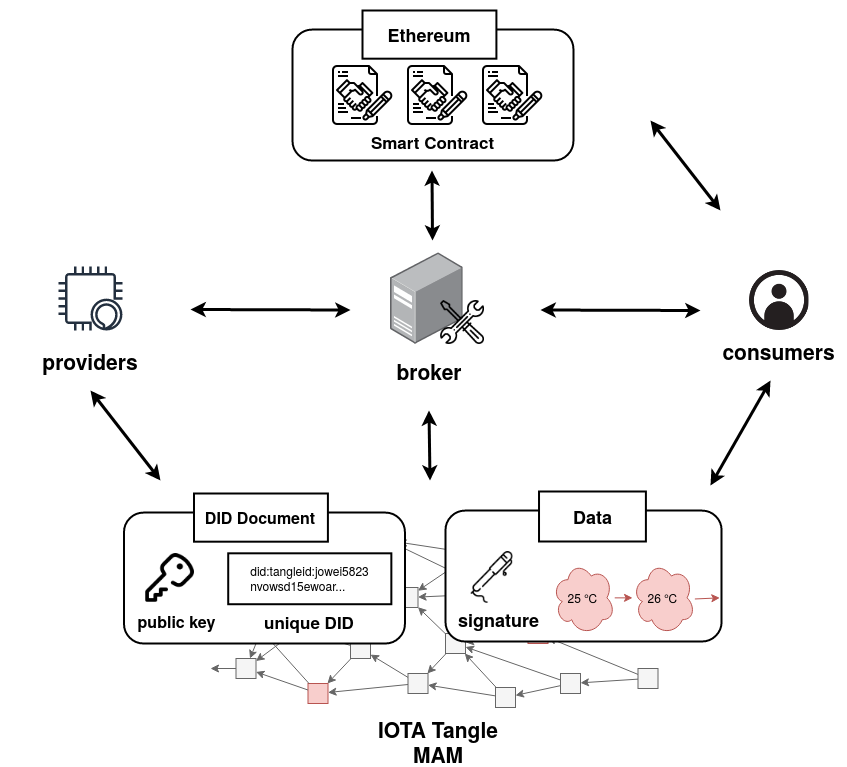
\includegraphics[width=3.in]{system_design}
    \caption{The system design of a decentralized data trading infrastructure which consists of data providers, consumers and brokers.}
    \label{fig:system_design}
\end{figure}

%TODO: cite IOTAIndustryMarketplace
\section{Related Work}
\label{section:relatedWork}
% pub/sub
\subsection{The Publish/subscribe Communication Models Over Blockchain}
The pub/sub service model consists of publishers, subscribers, and brokers, which has been proven\cite{pubSubAnalysis, pubSubAnalysis2} to be an efficient and flexible solution for a large number of diverse entities like IoT applications. A lot of work in the pub/sub system built on top of blockchain focused on the reliability, scalability, and the different security issues such as, encrypted data communication, privacy-preserving data subscription, and access control of the digital asset.

M. B. Abdullahi and G. Wang\cite{centralPubSub} presented a secure pub/sub data storage service in Wireless sensor networks (WSNs) which ensures several security issues. Each user has an identity for authentication, whereas subscribers' interests are encoded before matching to protect users' interests. Additionally, the proposed encryption scheme can prevent adversary to access published data if the sensor node is compromised. However, the access control and encryption keys of data are enforced by the network controllers (NCs) and CAs, which may be a potential security risk of the system, e.g., single-point failure. G. S. Ramachandran et al.\cite{trinity} pointed out the security risk of centralized brokers and applied DLTs to build a distributed pub/sub system that promotes the transparency of interactions of participants and the status of data. With the help of the Ethereum smart contract, users can perform data validation easily, and brokers can keep track of data status. But data is plaintext on blockchain, in which the privacy problem of sensitive data needs to be considered carefully.

In \cite{userCentricData}, the publisher runs a node in blockchain that preserves all the history data of the ledger, therefore, they can publish and manage data without any third-parties. The subscribers request publisher directly and ask them to save a cache space for interesting data. The main contribution of the system is to ensure data owners have full controls of produced data, but the data owners need to have well devices and environments to perform such functionalities and preserve data. Also, the rights for accessing digital assets are more compatible in the IoT scenarios instead of copying raw data. Secure Pub-Sub model\cite{SPS}, a brokerless of pub/sub model, is proposed to eliminate the security risk of middleware in the model and to provide a reputation-based fairness payment strategy on blockchain. The privacy and data security are considered thoroughly with the encryption scheme, while the reputation of publishers, payment, and data sharing are deployed on smart contracts that allow all operations are transparent. The reputation system and the punishment rules against malicious acts of subscribers and publishers. Yet, without brokers, providers and subscribers may need to reveal more sensitive information like IP address in order to match both sides. Another broker-less model in \cite{PrivacyPreservPubSub} protects the subscribers' privacy by encrypting users' interests with the light-weight PKEwET\cite{PKEwET}, which allows publishers to match the subscribers' interests in the ciphertext.

The previous works contribute to different aspects of building a reliable pub/sub system over blockchain. However, a few work propose an overall thinking of the pub/sub system, which ensures the privacy of players, preserves data securely and make data trackable, which is a vital consideration for IoT and mobile computing across organizations, and even stimulates data economics.

\subsection{Trusted IoT Trading Infrastructure}
Multiple infrastructures for trusted IoT data trading have been proposed by Paolo Missier et. al\cite{MindMyValue} presenting an IoT brokered infrastructure based marketplace that enables trading with Ethereum smart contracts. The brokers are only responsible for data transmission in order to adapt flexible agreement between participants. Unlike the standard pub/sub model that matches publishers and subscribers that participants are unaware of each other. However, the data cubes (i.e., a tuple of information, such as provider, subscriber, and time period) are stored in a centralized Cassandra NoSQL database, which is guaranteed to be tamper-proof but the risk of single-point failure still exists.

A. Colman et al. \cite{TrustedMarketplaceWearable} discussed on trading the sensitive data among wearables. Several security issues are well discussed and solved with DLTs in the paper, the system consists of multiple components aiming for different responsibilities, such as data anonymizer eliminates keen information for privacy protection, access controller handles the key management and contract manager manages Ethereum smart contracts. While the trading processes are split into multiple servers, and the request/response communication model is applied, the scalability problem of the marketplace remains.

In the following researches, Masked Authenticated Messaging (MAM)\cite{MAM} is regarded as a secure data transmission layer and data storage built on top of DLT which provides access control, tamper-proof and authentication functionalities by tailoring messages to a channel. Jinzhi Lu et al.\cite{luDecentralizedDM} builds the data exchange system with MAM and IPFS\cite{IPFS}, a content-based addressing distributed storage system. Considering the limited transaction processing capability of DLT, the authors suggest to adopt IPFS to handle the encrypted large data sets, then add the encrypted IPFS link to MAM for further exchange. This research takes MAM as a data transmission layer only that focuses on secure data exchanging architecture design and security analysis, but the trading strategies are not studied yet. A similar infrastructure proposed by Zichichi et al.\cite{SocialGood} offered key and entry points management with MAM that minimizes the information which data producers need to hold. Also, Ethereum smart contract is used to maintain an authorized user list and to enable trading. However, the access control is examined by Authentication Service, the only client/server communication architecture, where the security issues and bottleneck of the system emerges from, and the details of trading and interactions between providers and consumers are not illustrated in this paper. Though taking IPFS as data storage instead of MAM is more efficient due to the current growth of underlying DLT, the chance of data losses and the efficiency of IPFS remain, which will be further discussed in Section.~\ref{section:distributed_storage}.

The researches below adopt MAM as data storage and a secure data transmission layer. The industrial data marketplace\cite{IOTAIdustryMarketplace} proposed by IOTA Foundation targets for IoT data streams trading. Service requesters call for proposals of interested data and accept/reject proposals from service providers. After a proposal is accepted, the requesters can access data streams stored via MAM and pay providers in IOTA tokens. This proposal matching and the trading procedure can be automated without any human guidance\cite{IOTAIdustryMarketplaceWithoutHuman}. Nevertheless, this trading model does not take into account the refund and unsubscribe mechanism, the service requesters still need to pay even if they want to unsubscribe or the data does not meet expectations.

O. Lamtzidis and J. Gialelis \cite{IOTASensorNode} proposed a distributed sensor node system to exchange data and establish a data monetization economy paradigm. The Back-End server helps sensor nodes to accelerate data uploads to MAM, manages keys and metadata of data streams, and evaluates data price according to its quality. Furthermore, the Back-End server operates a user-friendly interface of the marketplace and tackles all trading procedures. The heavy loading of Back-End server encounters the system scalability problem, single-point failure as well as malicious attacks which may damage the profits of all players. And the pricing strategy allows buyout but does not take subscribe/unsubscribe based diagrams into consideration. The decentralized data marketplace in \cite{DDMSmartCities} is fully decentralized without the existence of any intermediate server but data providers only, data providers attach, and trade data streams via MAM. With MAM, the data streams subscription is enabled, yet the conditions and details like refund and unsubscription are not discussed in this paper.
 
\subsection{Distributed Storage System}
\label{section:distributed_storage}
Decentralized storage systems allow users to store files in a distributed network that is maintained by individual nodes around the world instead of a central service provider. Nevertheless, DLTs are often used as the backbone of these systems like data storage and also an incentive layer to encourage people to get involved in the network.

Filecoin \cite{FileCoin} in the Inter-Planetary File system (IPFS) is an incentive layer to incent nodes to provide storage. IPFS is a content-based addressing storage model in a peer-to-peer network, in which users can obtain the data with the unique hash value through the network. Furthermore, considering the data may lose in the network, IPFS provides \textbf{pin} command for users to store the contents locally that will not be removed. However, the IoT sensor devices have limited space which is not appropriate to preserve generated data. Also, users can have a hard time finding the contents quickly if data is not widely available, and the large amount of IPFS nodes and contents. Thus, several pinning services like Pinata provide multiple IPFS nodes around the world to pin users' contents and charge by the size and replicas of contents, and users can even join the dedicated network to speed up the retrieving process. Nevertheless, the efficiency problems still occur if the dedicated network grows larger.

Sia\cite{Sia} splits the uploaded file into multiple data segments encrypted with the owner's private key, then ciphertext is sent to the Sia nodes that rent the storage in Siacoin through smart contracts. Files are duplicated in multiple nodes to prevent data loss.

\section{System Design Thinking}
\label{section:design_thinking}
\subsection{Data subscription-based trading platform players}
There are three major roles, data providers, data consumers, and brokers which are similar to the pub/sub messaging model. But unlike the standard pub/sub model where brokers link the publishers and subscribers who are not aware of each other, in our proposed architecture, the brokers are only responsible for message delivery and essential verification processes. As shown in Fig.~\ref{fig:pub_sub_model}.

\begin{figure}[!t]
    \centering
    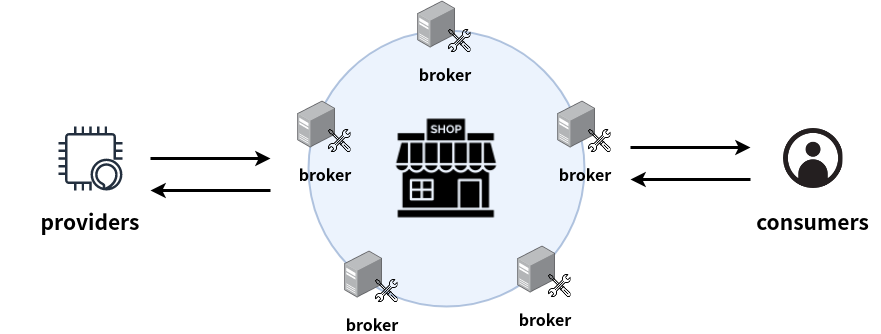
\includegraphics[width=3.5in]{pub_sub_model}
    \caption{The players in data subscription-based trading platform consists of data providers, data consumers and brokers.}
    \label{fig:pub_sub_model}
\end{figure}

\begin{itemize}
\item \textbf{Data Provider: }
Data providers are the ones that generate streaming data and set the data price based on the different types of data. Subscription fees can motivate data providers to maintain and improve the quality of data.
\item \textbf{Data Consumer: }
Data consumers are entities that are willing to buy data streams. As it is laborious to widely deploy devices to collect data from scratch and it is also difficult to find desired data sets, purchase is the fastest and efficient way to get the desired data sets.
\item \textbf{Broker: }
Brokers are responsible for building an agreement between data providers and consumers. Brokers are required to be online for providers and consumers, and they are incentivized by charging brokerage fees.
\end{itemize}

We adopt the brokered infrastructure for three reasons. Firstly, it inherits the benefits from the standard pub/sub model which is more efficient than the request/response model specifically in a large scale system. Furthermore, if either side is offline, the proceeding tasks have to stop and start over. With brokers, the unfinished work can be cached or accomplished. Second, a fully decentralized architecture has difficulties to brings data providers and consumers together, both of them need to reveal more sensitive information, such as IP address, in order to build the communication tunnel. The existence of brokers resolved the privacy issue, as brokers are the bridges that link data providers and consumers, participants can trade with minimum information like its identifier and public key. Third, a refund process needs brokers to host and supervise the procedures in order to protect the rights of participants, which will be further discussed in Section.~\ref{section:refund}.

\begin{figure*}[!t]
    \centering
    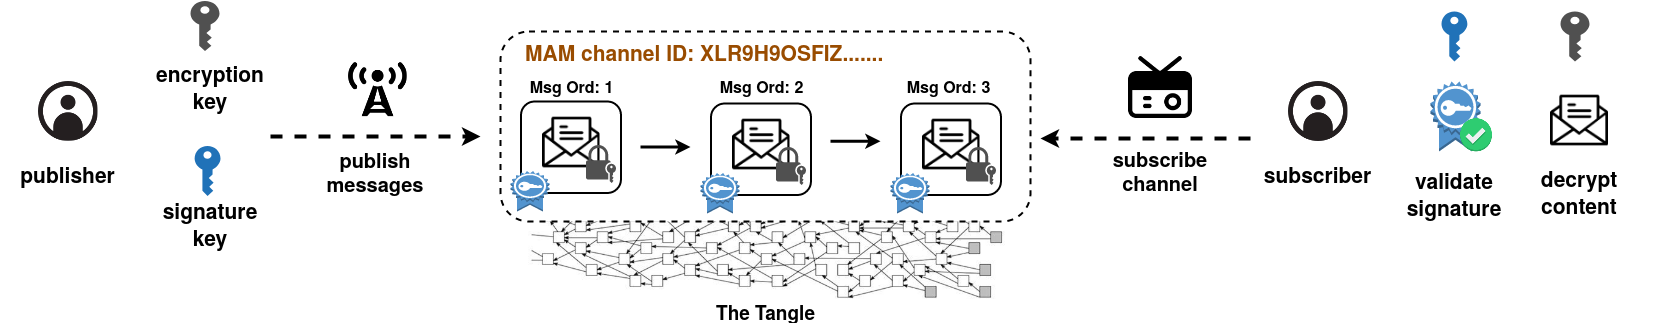
\includegraphics[width=\linewidth]{channel_and_key}
    \caption{Within MAM channel, the message publisher has 2 types of key, an encryption key for encrypting contents and a signature key per message for digital signatures. Subscribers can validate the message with signature keys and decrypt messages with encryption keys.}
    \label{fig:channel_and_key}
\end{figure*}


\subsection{Choice of Data Storage}
Data storage is the trust basis of data trading platforms where the data assets are reserved. Streaming data unlike a fixed set of data that can be verified by the hash of the whole pack of data, it consists of continually granular records of each time slot. Therefore, the verification such as, data integrity and source identity is narrow down to a data point as well. In our proposed architecture, we adopt MAM as data storage to resolve the challenges of managing and verifying data streams. MAM is the second layer data communication protocol built on top of IOTA\cite{IOTAwhitepaper} network, the Tangle, a feeless cryptocurrency designed for IoT, which introduces properties like publishing, classifying and tracking authenticated message streams. Carrying these properties, MAM is also appropriate for building a self-sovereign identity system where the identity information such as public key, unique identifiers of services and metadata are stored. One can easily prove himself by sharing the identifier on MAM without any authority.

Currently, considering the efficiency of uploading large files, IPFS performs better than MAM (i.e., writing contents to IOTA network). However, IOTA network scales when more users and transactions join, and the MAM operations can be delegated to powerful proxy servers which is illustrated in Section.~\ref{section:ta_endpoint}. Furthermore, adopting IPFS in IoT scenarios may meet the challenges of data loss and data retrieving efficiency.

In our work, MAM builds the trust of the platform while meeting the requirements of data trading which can be concluded below:

\begin{itemize}
    \item \textbf{Scalability}:
    \begin{itemize}
        \item Benefits from the underlying Tangle network, the system scales when more participants and more transactions join the network.
        \item For both data providers and consumers, MAM keeps the number of managed keys and data entry points as small as possible
    \end{itemize}    
    \item \textbf{Integrity}:
    \begin{itemize}
        \item Messages published to the Tangle are tamper-proof against malicious modification.
        \item Messages are signed with the keys pre-generated under Merkle signature scheme\cite{MSS} (MSS) that both keys and messages can be verified by participants.
    \end{itemize}
    \item \textbf{Confidentiality}:
    \begin{itemize}
        \item The encrypted data are uploaded that only participants that have keys can decrypt.
        \item The authorized users can retrieve data streams since data is written on the Tangle which can be queried as long as the IOTA network is alive.
        \item MAM provides forward-secrecy. The entry points of future data can be derived, but it's impossible to trace back those in the past. This feature prevents adversaries from retrieving published history even if the key is revealed.
    \end{itemize}
\end{itemize}

MAM publishes authenticated streaming data to channel and endpoint as zero-value transactions to the Tangle and provides the ability to publish and fetch encrypted messages over the network along with data integrity and access control. The payload of a MAM message can be encrypted with an \textbf{encryption key} that restricts only authorized players can access contents, the ciphertext is then signed with \textbf{signature key} generated with MSS and attached to the Tangle. This approach allows users to validate the signatures without knowing the actual contents but ensuring the messages do come from the exact source. See Fig.~\ref{fig:channel_and_key} for illustration.

Using MAM as a data storage benefits from the scalability of the underlying IOTA network as well as the decentralized and fault-tolerant characteristics of distributed ledgers, which reduce the risks of centralized storage services. Furthermore, the rights of data access are traded instead of a copy of data in the trading platform, which eliminates the need for data consumers to have additional storage.

\subsection{Digital Identity}
The digital identity represents entities and holds the digital assets within the digital world, it is important to prove and show the identity to others during interactions. We select the decentralized identity model rather than a centralized one for the concerns in Table.\ref{tab:did}.

\begin{table}[h]
    \caption{The comparison of centralized and decentralized identity model}
    \label{tab:did}
    \begin{tabularx}{\linewidth}{|l|X|X|}
    \hline
        \textbf{Identity Model} & \textbf{Centralized} & \textbf{Decentralized} \\
        \hline
        Control & Enterprises control identities & Entities control their identities \\
        \hline
        Security & Identity held in a centralized service is a honeypot for cyber attacks & Decentralized identity limits data exposure \\
        \hline
        Portability & Identity is fragmented across enterprises & Identity can be portable across enterprises \\
        \hline
    \end{tabularx}
\end{table}

The centralized identity model may have the single-point failure in identifier management and security issues like data leakage. With sensitive information holding on certain authorities, the leakage caused by cyber-attacks or unscrupulous organizations trading user data damage the users' privacy. Furthermore, having a recognizable and portable identifier is important, otherwise, it is hard to cooperate fragmented identities of different data formats among institutions, and organizations may not approve identifiers of others. The decentralized identity model give back the controls of data to users that can resolve the aforementioned concerns in the centralized one.

In the decentralized identity model, every entity has a Decentralized Identifiers (DID\cite{DID} defined by W3C that contains identity information such as public key, unique identifiers of services and metadata. The digital footprints of entities are made up of Verifiable Credential (VC) added to their DIDs, issued by trusted issuers, such as schools and government departments. If a VC is verified via the issuer's public key, the message will be labeled as trusted. Fig.~\ref{fig:did_vc} shows the relationship of VC issuer, verifier and user.

\begin{figure}[h]
    \centering
    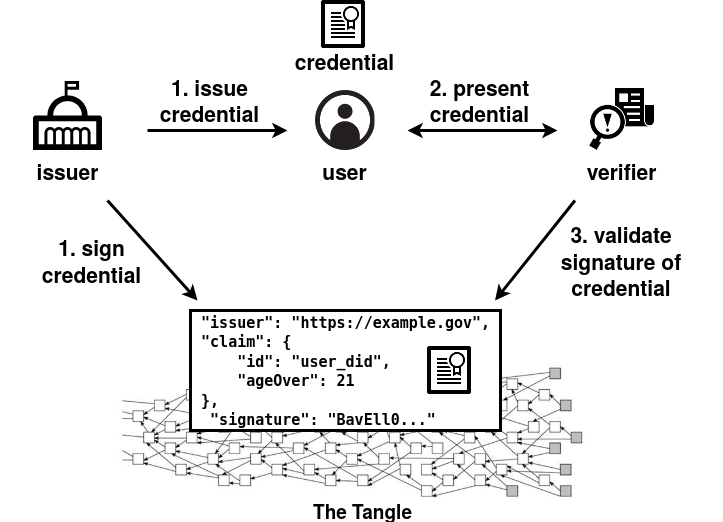
\includegraphics[width=3.in]{DID_VC}
    \caption{The trusted issuer requests user's DID, then issues a VC with his/hers signature. The user can then present the VC to verifier for signature validation.}
    \label{fig:did_vc}
\end{figure}

In our architecture, a decentralized identity system TangleID\cite{TangleID} is used, which is built on top of MAM where change logs of DIDs are traceable. One can easily prove himself by sharing the identifier on MAM without any authority.

Through TangleID, entities get a public/private key pair, the location of the DID document, and the seed (i.e., the identifier of its owner in IOTA) that used to generate the DID document MAM channel. The public/private key pair can be used to exchange sensitive data and establish trust communication, where messages that are encrypted with a public key can only be decrypted with the private key owner. During data subscription process, the encryption keys of data products are encrypted with data consumers' public key on the DID document which ensures only the subscribed consumers are accessible. See Fig.~\ref{fig:TangleID}

\begin{figure}[h]
    \centering
    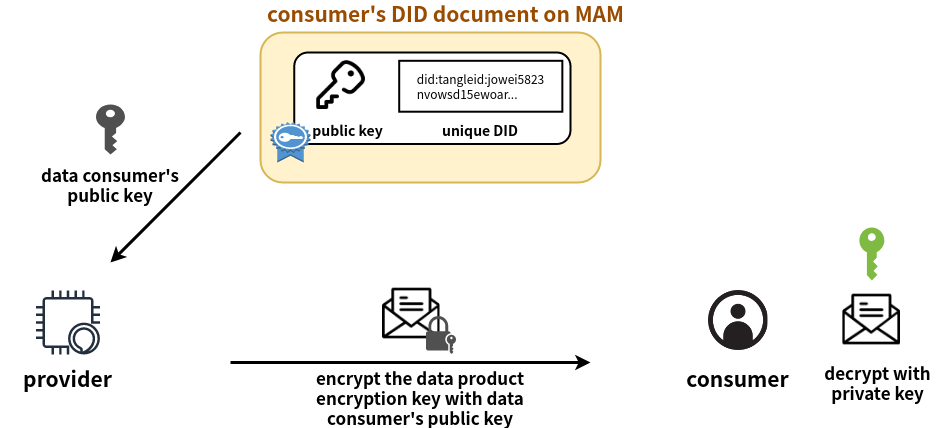
\includegraphics[width=3.5in]{TangleID}
    \caption{To participate in the data trading, players are required to have DID document issued by TangleID. The consumer first needs to send a registration request to TangleID to get the MAM channel ID of the DID document and a public/private key pair for authentication. When the trade establishes, the consumer sends the DID MAM channel ID to the provider in order to perform encryption key exchange. The data provider can then retrieve the consumer's public key and encrypt the content with it. After the consumer gets the encrypted message, he/she can decrypt the ciphertext with the private key and finally get the encryption key of data product.}
    \label{fig:TangleID}
\end{figure}


\subsection{Enable Automated Trading Process}
\begin{figure*}[t]
    \centering
    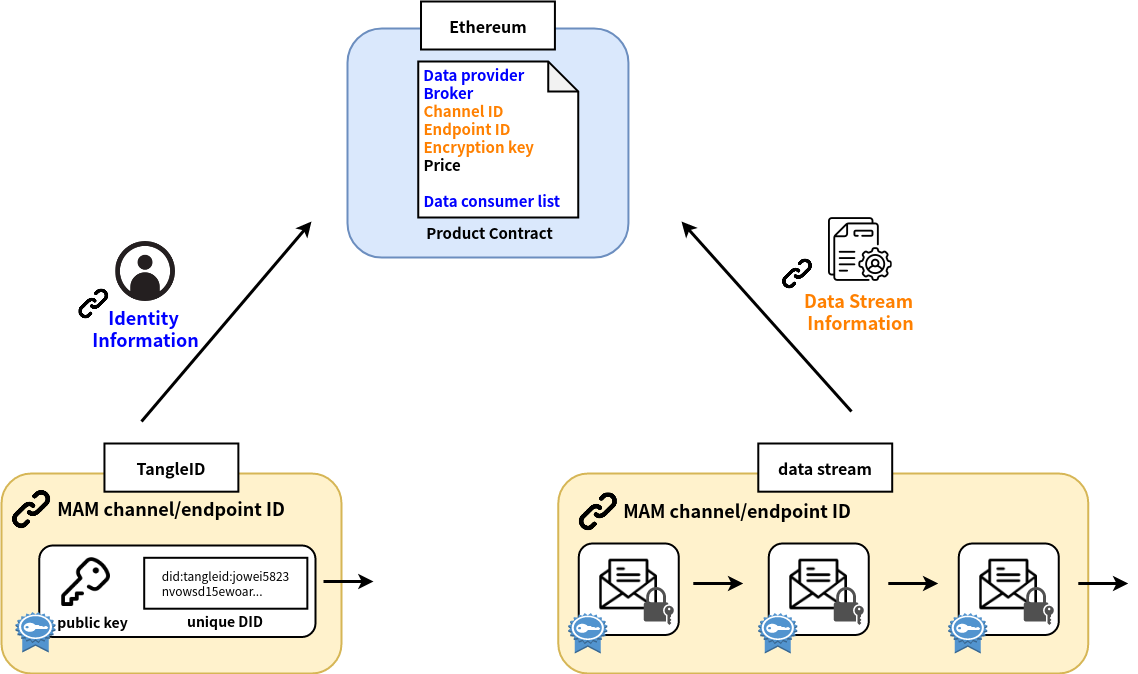
\includegraphics[width=4in]{smart_contract_mam}
    \caption{The information of identity and data streams are stored on the Tangle with MAM which is all recorded on Product Contracts. Participants can easily retrieve information via the Product Contract and proceed to trade. For signature validation check and further exchange encryption keys, the MAM channel ID of participants' DID document are written down, presented in blue color. The orange color stands for the information of data products, which includes the data stream channel/endpoint ID.}
    \label{fig:smart_contract_mam}
\end{figure*}

Ethereum is a cryptocurrency building on top of a public blockchain-based distributed ledger. It provides the smart contract, which is a protocol for formulating agreement on a blockchain that running on decentralized virtual machines. A smart contract can interact with other contracts, make decisions, store data, and transfer cryptocurrency. All the participants in Ethereum can verify and execute the contracts, and once the contract is triggered, it is uninterruptible and will be executed automatically without any third-parties.

With the functionalities of Ethereum smart contracts, a flexible and verifiable trading mechanism can be achieved. In our system, \textbf{Product Contract} is made for the product launching and subscribing. The information on data products such as the address of the data provider, subscription fee, brokerage fee, the threshold of consent votes of refunding, MAM channel/endpoint ID (the data entry point), time period, and the broker-verified encryption key are listed on Product Contract. Listing. \ref{lst:constructor} list the data fields of Product Contract, and Fig.~\ref{fig:smart_contract_mam} shows the relationship of Product Contract and MAM.

Furthermore, the participants can exchange encryption keys without any authorities via smart contracts. Though this design may cost extra transaction fees than exchanging key off-chain, it is considered a more secure strategy to protect the privacy of participants that only the DID document address and Ethereum addresses are revealed during the subscription process. Binding trading and data storage to smart contracts ensures consumers can always have access after payment, even if the key is lost, and providers can track and manage the authorized user list.

The transparency of smart contracts brings advantages for data providers and consumers. One of the advantages is that the trading states and progress are visible and verifiable which profits providers and consumers respectively. For data providers, with every detail opened, the consumer list functions like a reputation evaluation, the better the quality the more the consumers he/she has, which are also reputation references for data consumers. The enforcement of smart contracts also ensures the rights of participants that they fulfill the agreed contract under any circumstances.

\lstdefinestyle{solidity}{
    captionpos=b,
    tabsize=4,
    basicstyle=\scriptsize
}
\lstset{style=solidity}
\begin{lstlisting}[caption={Product Contract data fields}, label={lst:constructor}, frame=single]
contract Product {
    address public broker;
    address public provider;
    bool isBrokerWithdraw;
    bool isProviderWithdraw;
    address[] consumers;
    
    struct Purchase {
        bool affirmativeVote;
        bool isConsumerWithdraw;
        bool isKeyAdded;
        bool isSubscribe;
        string encryptKey;
    }
    mapping(address => Purchase) public consumer2Purchase;
    
    uint public price;
    uint public totalAmount;
    uint public brokerage;
    uint public cancellation;
    uint public threshold;
    string public channelRoot;
    string public endPoint;
    uint public totalNumber;
    uint public uploadedNumber;
    uint public affirmativeVotes;
    string hashedKey;
    string certifiedKey;
    
    enum State {Launched, KeyCertified, Finished, Refunded}
    State public state;
}
\end{lstlisting}

\subsection{Enable computation tasks delegation to broker with privacy}
To manage data products and to benefit from trading, data providers have to interact with MAM and Ethereum smart contract while doing its original tasks. However, the limited resources of low-level devices should be used in their jobs instead of handling all trading processes. Therefore, the operations of MAM and smart contracts are better to be delegated to brokers. The delegation should ensure the privacy of data providers, for instance, brokers are asked to attach messages to MAM and record encryption keys to smart contracts without knowing the contents. The encryption key upload procedure is illustrated in Section.~\ref{section:launch_data_product}.

As for MAM operations, the performance results in Section.\ref{section:mam_performance} show that operating MAM costs a lot of resources for the devices, therefore, we present an alternative solution for data providers to delegate these computing tasks to powerful proxy servers, Tangle-accelerator\cite{TA}, while ensuring the privacy. The details would be further illustrated in Section.\ref{section:ta_endpoint}.

\section{Masked Authenticated Messaging}
\label{section:MAM}
MAM enables broadcasting encrypted and authenticated data stream, referring as a channel, on the Tangle. The publisher publishes messages that are propagated through the network and can be accessed by the subscribers only. With MAM, the rights of data access are traded instead of a copy of data in the trading platform, which eliminates the need for data consumers to have additional storage.
Section.~\ref{section:mam_streams} to ~\ref{section:mam_features} explain the structure, fuctions and features of MAM proposed by IOTA Foundation, and our proposed MAM delegation mechanism is clarified in Section.~\ref{section:ta_endpoint}.

\subsection{The Message Streams}
\label{section:mam_streams}
A channel/endpoint is a stream of MAM transaction bundles, which consist of signature and the masked message payload. To publish a MAM message to a channel, MAM deploys MSS to sign the message payload to the channel, where $channel\ ID = root$ i.e., the MSS Merkle root. The Merkle tree is generated with \textbf{seed}, an identifier of its owner in the IOTA protocol, represents the ownership of all things associated with the user in the IOTA ecosystem. Furthermore, the structure of channel/endpoint implements forward linking, each address of a message can be derived from the previous one that other entities can fetch the next payload. This design also brings the advantage of forward secrecy, where no one has access to the data back from his/her entry point. Figure.~\ref{fig:mam_structure} shows the structure of the MAM channel/endpoint.

\begin{figure}[h]
    \centering
    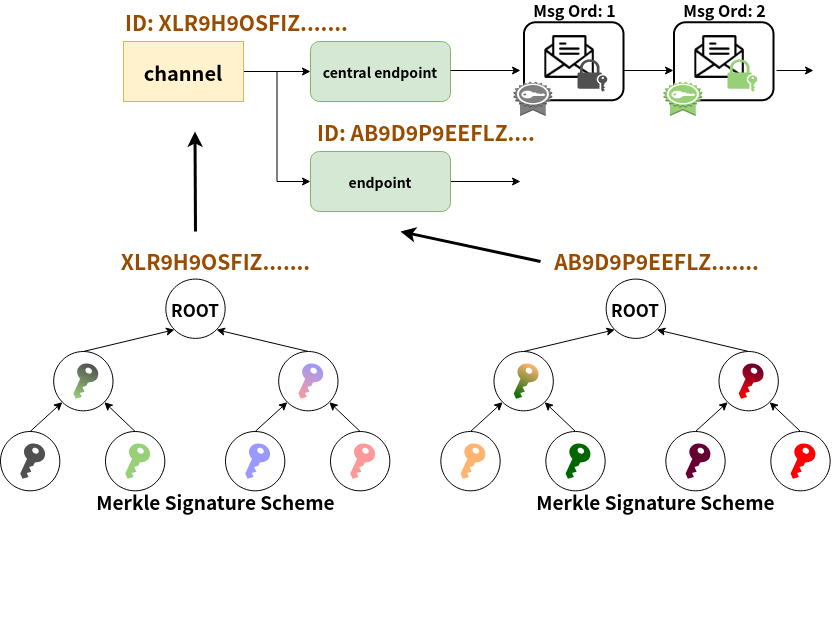
\includegraphics[width=3.5in]{mam_structure}
    \caption{With a seed, users can generate multiple channels, which can then generate multiple endpoints. The IDs of channel and endpoint are the roots of different Merkle trees in MSS. The "central endpoint" are endpoints that has ID, where $endpoint\ ID = channel\ ID$.}
    \label{fig:mam_structure}
\end{figure}

\subsection{Enable Access Control and Authentication}
\label{section:mam_functions}
The access control can be enabled via encryption with NTRU\cite{NTRU}, a quantum secure cryptosystem, or Pre-shared key (PSK), to prevent random users retrieving the data from channels. If the message payload is encrypted, subscribers are required for encryption keys to decode messages. The authentication in MAM includes two aspects: source and data. Source authentication ensures the message that originates from the claimed owner, and data authentication ensures the integrity of the data from the sender. These are achieved through the MSS and One-way hash functions by validating the signature added in the signature section of the MAM bundle. However, the size of Merkle Hash Trees, that is, the size of a channel/endpoint should be determined at the start. Thus, data providers need to first decide how to distribute data products into MAM channels/endpoints before uploading data.

\subsection{The Advantages of Adopting MAM in Subscription-based Data Trading Infrastructure}
\label{section:mam_features}
%scalability
\subsubsection{A Scalable Keys and Data Entry Points Management}
The importance of scalable key and data entry points management increases over time. In MAM, with an entry point (i.e., the address of transaction) and the encryption key, one can derive the following addresses of the transaction and retrieve data. To manage a data stream, the owner only needs to preserve 1 entry point and 1 encryption key in MAM, but $N$ entry points and 1 encryption key in other distributed storage.

%classify
\subsubsection{Data Streams Classification and Traceability}
The channel and endpoint structures enable users to be able to easily categorized data streams with respect to different types and usages. For instance, sensor devices like AirBox\cite{LASS}, collect environmental data, can split the statistics like PM 2.5 and humidity by time period into separate channels, which is useful for data providers to organize records and to pack into different data products. As for data traceability, users can easily track the footprints of data change logs as well as checking the validity of modifications with the signature.

\subsection{Delegate MAM operations to Tangle-accelerator}
\label{section:ta_endpoint}
MAM builds a secure and authenticated communication protocol on top of multiple cryptosystems, which low-level devices need to spend a lot of resources to apply it, and they may not even support built-in libraries in the regular operating systems. To overcome these concerns, we propose another approach that allows data providers to delegate the MAM operations to Tangle-accelerators, proxy servers with high computation power, which can accelerate the interactions with Tangle while ensuring the privacy of data providers. Fig.~ \ref{fig:ta_struct} shows the structure of Tangle-accelerator, and Fig.~\ref{fig:delegation} shows how data providers can adopt MAM.

\begin{figure}[!t]
    \centering
    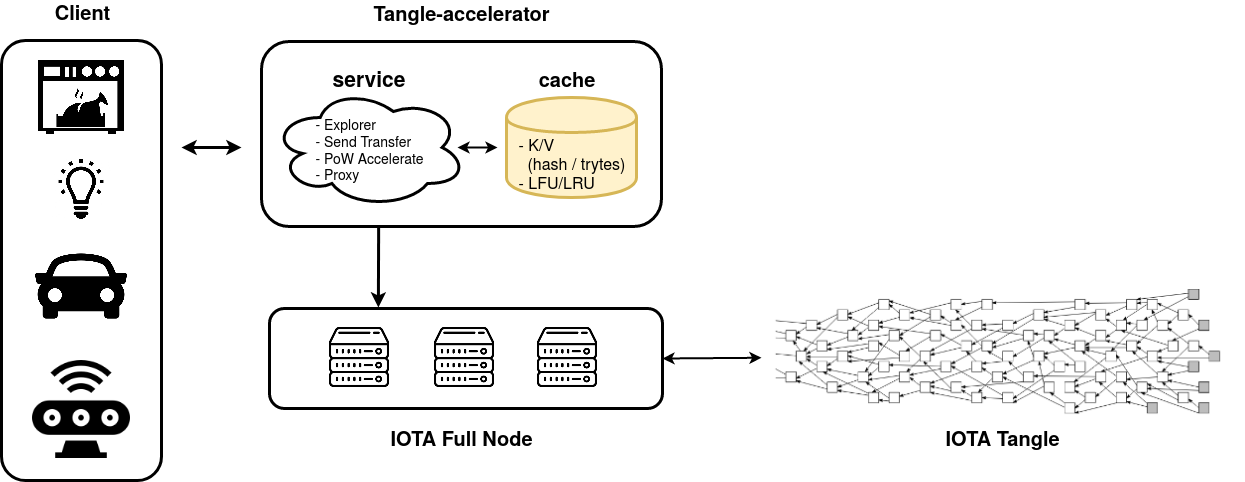
\includegraphics[width=3.5in]{ta_structure}
    \caption{Tangle-accelerator distributes IOTA API requests to idle IOTA nodes (i.e., full nodes) and provides Proof-of-Work acceleration. It can also cache the requests/responses in a key-value store to shorten response time, and automatically resend requests if failed. Tangle-accelerators also form a firewall for full nodes, which don't need to reveal the IP address to public and reduce the risks of being attacks.}
    \label{fig:ta_struct}
\end{figure}

\begin{figure}[!t]
    \centering
    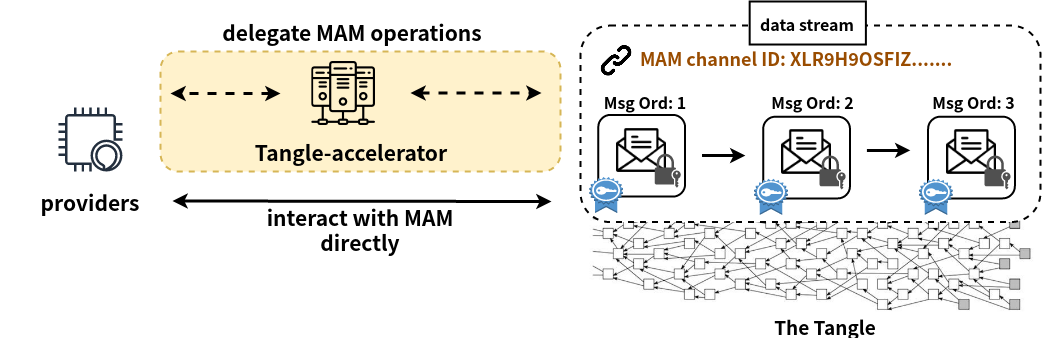
\includegraphics[width=\linewidth]{delegation}
    \caption{Data providers can use MAM in 2 ways: the provider performs MAM operations locally, and the provider delegates MAM operations to Tangle-accelerator.}
    \label{fig:delegation}
\end{figure}


\subsubsection{Communication Protocol}
In the following sections, we refer to the low-level devices as \textbf{endpoint}s. MQTT\cite{MQTT} is chosen as the communication protocol, which requires fewer TCP packets and less traffic. The topic-based pub/sub pattern and lightweight packet that MQTT adopts would undoubtedly play an important role in endpoints with limited bandwidth. The pub/sub model decouples publishers and subscribers in many ways:

\begin{itemize}
    \item Space decoupling: Both publishers and subscribers don't need to know each other.
    \item Time decoupling: Publishers and subscribers do not need to be active at the same time.
    \item Synchronization decoupling: Operations are decoupled from the publishers and subscribers. The publishers do not need to be alive until the response arrives. Messages from the publisher can be served as send-and-forget fashion.
\end{itemize}

\subsubsection{End-to-End-Encryption}
Introducing a proxy server to process all the cryptographic operations causes the proxy server or the middle man can easily tamper the message. To avoid such malicious operations during transmission, we introduce another lightweight end-to-end-encryption (E2EE) upon MAM protocol. The plaintext will be encrypted with this lightweight end-to-end-encryption. The E2EE process ensures only authorized subscribers can read the messages published on MAM.

%pic
\begin{figure*}[!t]
    \centering
    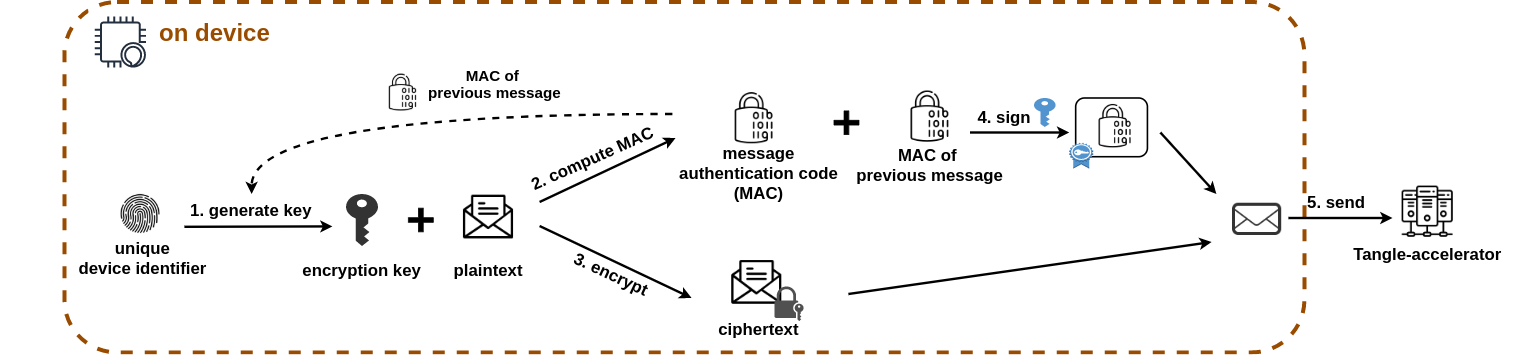
\includegraphics[width=\linewidth]{MAM_E2EE}
    \caption{The process of E2EE.}
    \label{fig:MAM_E2EE}
\end{figure*}

In the Fig.~\ref{fig:MAM_E2EE}, we illustrate each step in the presented E2EE process. The details of the steps are addressed below:

\begin{enumerate}
    \item Generate symmetric keys with the unique device identifier and Message Authentication Code (MAC) of the previous message. If the message is the genesis message, then sharing secret initialization information would serve as the MAC of the previous message. Key Derivation Function (KDF) is used to generate the symmetric keys.
    \item Compute the Message Authentication Code (MAC) of current message with the Hash-based Message Authentication Code(HMAC). Both plaintext and symmetric key would be given as parameters in HMAC.
    \item Apply the generated symmetric key to encrypt the plaintext.
    \item Concatenate the MAC of the current message would and the MAC of the previous message, and then the result will be signed with a digital signature algorithm.
    \item Send the ciphertext along with signed MAC.
\end{enumerate}

\begin{table}[htbp]
    \caption{AES256 Encryption Performance Numbers}
    \label{tab:AES_NI}
    \begin{center}
        \begin{tabular}{ |c||c|c|c|  }
            %\hline
            %\multicolumn{4}{|c|}{} \\
            \hline
            Size& \makecell{NON AES-NI \\ (msecs)} & \makecell{AES-NI \\ (msecs)} & \makecell{Encryption \\ Acceleration (\%)} \\
            \hline
            50 MB  & 1026  & 563   & 45.13 \\
            100 MB & 2036  & 1297  & 36.30 \\
            200 MB & 4282  & 2984  & 30.31 \\
            512 MB & 10754 & 6401  & 40.48 \\
            1 GB   & 23976 & 15721 & 34.43 \\
            \hline
        \end{tabular}
    \end{center}
\end{table}

The E2EE protocol presented in this paper combines a series of different cryptographic procedures. Each of them can be chosen on the basis of the working hardware and scenario by developers. On certain devices, hardware acceleration would be supported. With hardware-acceleration, the elapsed time could be dropped a step more. For example, applying AES-NI can accelerate AES operations around 40\% on Intel devices.\cite{AES-NI-Acceleration} According to Intel, Table~\ref{tab:AES_NI} shows the performance of Encryption of AES256 with and without hardware acceleration.

\subsubsection{Register with Tangle-accelerator}
Users with channel seed can acquire channel chain ownership. Seed is generated by unique hardware information on the edge device, so it should be transmitted to tangle-accelerator which allows it to publish messages on the MAM channel chain. Once the Tangle-accelerator receives the Seed from the edge device, it would return a unique user identifier that can be mapped to corresponding Seed when edge devices send requests. Asymmetric encryption is utilizing during the process of exchanging seed. The digital signature should be taken at the same time to ensure data integrity. Once the seed has been successfully exchanged, the edge device is successfully registered on the specific tangle-accelerator. Thus, the seed will not be exposed during communication after an edge device is successfully registered.

\subsubsection{Issues in End-to-End-Encryption}
E2EE helps a lot with low-level edge devices utilizing blockchain service. It dramatically reduces the execution time encryption takes. However, we met two challenges in the E2EE process:

\paragraph{Linear Time to Read Message}
It is linear time to decrypt messages instead of constant time. Nevertheless, there is one way to speed up the message decryption process. A subscriber can fetch multiple MAM messages with one API call, then the subscriber can decrypt the ciphertext at the local side. This procedure can reduce the time spending on internet communication.

\paragraph{Spam on Message Channel Chain}
Tampering the messages which have conducted E2EE would be a challenging mission. However, spamming would be the critical issue participants may meet under this architecture. It is risky for an edge device connects to a tangle-accelerator which is operated by unknown third-party. Sharing Channel Chain ownership with an unknown third-party would allow them to spam on the MAM Channel Chain. Spam would cause subscribers to waste plenty of time on decrypting useless messages. To prevent edge devices from the annoying attack, connecting to an known, trustworthy tangle-accelerator would be the easiest solution.

\section{Decentralized Subscription-based Data Trading Models}
\label{section:trading_model}
In this section, we illustrate how participants can join the data subscription platform, start subscribing, cancel subscription, and request refund.

\subsection{Prerequisite}
All participants are required to register on TangleID to get a DID document and public/private key pair for sensitive contents exchange and authentication. An Ethereum account is also needed to interact with smart contracts and transfer Ethereum tokens.

\subsection{Launch Data Products}
\label{section:launch_data_product}
To launch a data product, data providers need to create a MAM channel/endpoint for data streams and a Product Contract. For those resource-constraint IoT devices, the MAM related operations can be delegated to Tangle-accelerator, as mentioned in Section.~\ref{section:ta_endpoint}. And brokers are responsible for Product Contract creation.

The details of data products, such as data price, MAM channel/endpoint ID, and the length of data stream are listed on the Product Contract. As regard to the encryption key of data product, data provider computes the digest of sensitive contents with a hash function, and sends the digest as well as the signature to brokers. The broker can first verify the signature from data provider with the public key on the DID document. If it's valid, then the broker uploads the key; otherwise, the process will be aborted. Note that the broker needs to sign the encrypted encryption key he/she receives proving that it is uploaded by the responsible broker. This procedure allows data consumers to check whether the encryption key is uploaded by the committed data provider and broker before subscription. Furthermore, the encryption key can only be uploaded/updated under two circumstances: 1.) the new product launching. 2.) when data consumer unsubscribe to the product. Finally, the data product is launched and data providers can start uploading data. Fig.~\ref{fig:key_upload} demonstrates the key uploading process to the Product Contract via a broker. The product launching workflow is shown in Fig.~\ref{fig:launching_product} and Listing.~\ref{lst:key_certification} lists the Solidity codes of the key certification process.

\begin{figure}[h]
    \centering
    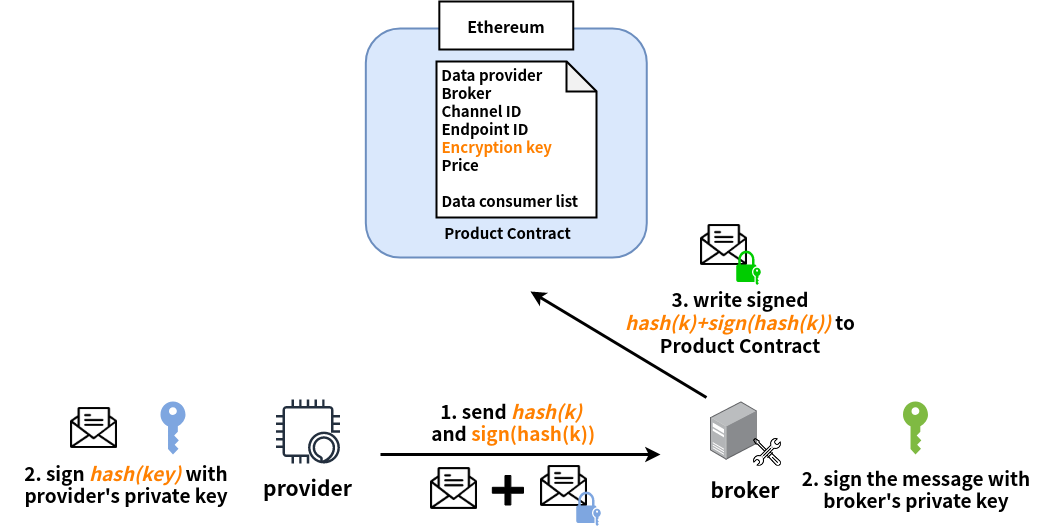
\includegraphics[width=3.5in]{key_upload}
    \caption{To add encryption key to Product Contract, the data provider sends the digest of the encryption key and the one that signed with his/her private key. After the broker receive the request, he/she performs digital signature as well to prove the encryption key is uploaded by the responsible broker, then writes the result to the Product Contract.}
    \label{fig:key_upload}
\end{figure}

\begin{figure}[!t]
    \centering
    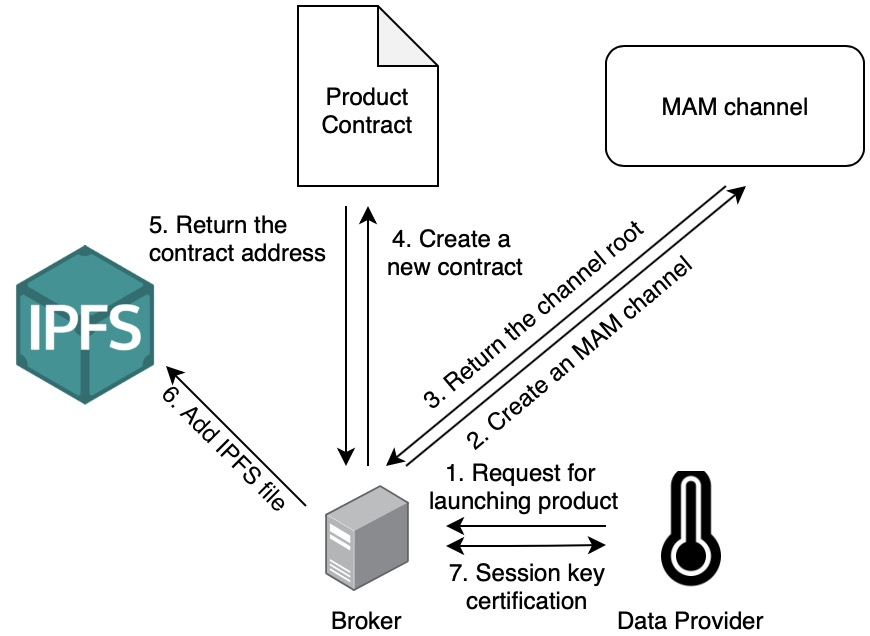
\includegraphics[width=2.5in]{launching_product}
    \caption{The process of launching a product.}
    \label{fig:launching_product}
\end{figure}

\begin{lstlisting}[caption={Functions of hased key update and certified key update}, label={lst:key_certification}, frame=single]
    function addHashedKey(
        string memory _hashedKey
    ) public {
        require(
            msg.sender == provider,
            "Only provider can add hashed key."
        );
        require(
            state == State.Launched,
            "One key has been certified."
        );
        hashedKey = hashedKey;
        emit newHashedKey(hashedKey);
    }

    function addCertifiedKey(
        string memory _certifiedKey
    ) public {
        require(
            msg.sender == broker,
            "Only broker can add certifiedKey."
        );
        require(
            state == State.Launched,
            "One key has been certified."
        );
        certifiedKey = _certifiedKey;
        state = State.KeyCertified;
        emit newCertifiedKey(certifiedKey);
    }
\end{lstlisting}

\subsection{Subscribe to Data Product}
Data consumers pay subscription fees to the Product Contract of desired data products, and data providers give the encryption key of data stream instead of the files to consumers. The MAM channel/endpoint encryption key is encrypted with the public key of data consumer by the data provider and written on the Product Contract, which ensures only data consumers can decode it via Product Contract.

Transferring the encryption key on smart contracts instead of off-chain not only ensures the consistency of the encryption key but also prevents frauds from malicious participants, and the exchange process is transparent to the public. Furthermore, with the help of brokers and smart contracts, both data providers and consumers do not need to be online at the same time to proceed with the trading process. The key sending process is shown in Fig.~\ref{fig:key_exchange} and Listing.~\ref{lst:key_exchange}. The subscription fee is transferred from the Product Contract to data providers when the committed data is available on MAM.

\begin{figure}[!t]
    \centering
    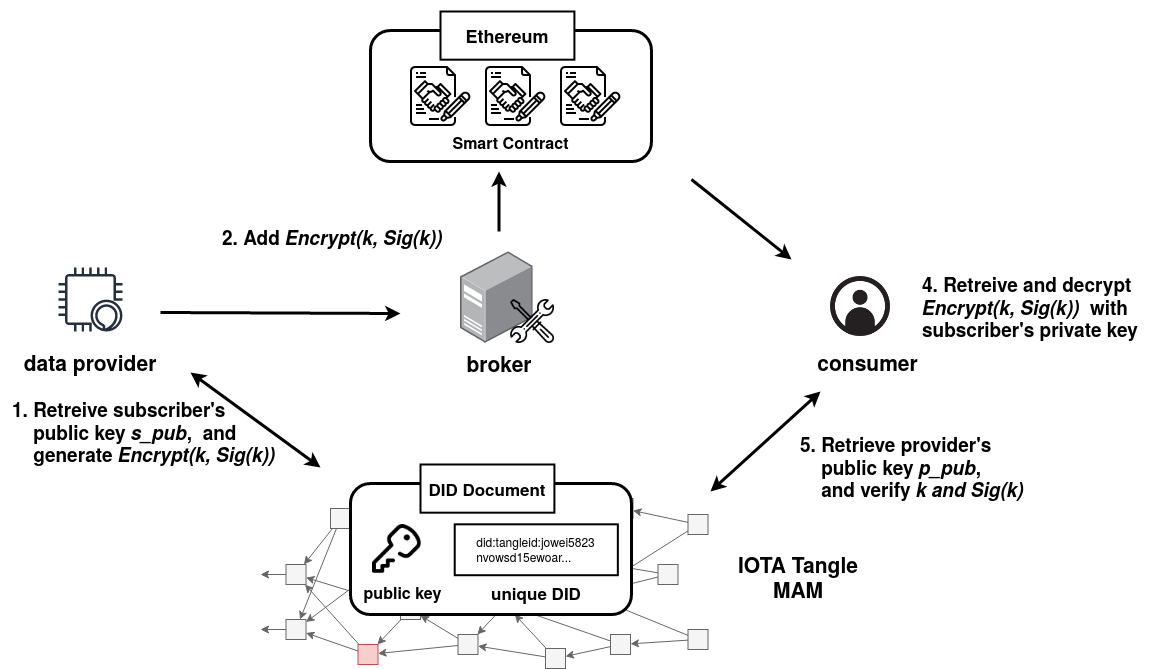
\includegraphics[width=3.5in]{key_exchange}
    \caption{Encryption key exchange process.}
    \label{fig:key_exchange}
\end{figure}

\lstdefinestyle{solidity}{
    captionpos=b,
    tabsize=4,
    basicstyle=\scriptsize
}
\lstset{style=solidity}

\begin{lstlisting}[caption={Add encryption key to data consumers}, label={lst:key_exchange}, frame=single]
function addEncryptKey(
    address _consumer,
    string memory _encryptKey
) public {
    require(
        msg.sender == provider,
        "Only provider can add the encrypted key."
    );
    require(
        consumer2Purchase[_consumer].isKeyAdded == false,
        "Encryption key has been added."
    );
    consumer2Purchase[_consumer].encryptKey = _encryptKey;
    consumer2Purchase[_consumer].isKeyAdded = true;
    emit newEncryptKey(_consumer, _encryptKey);
}
\end{lstlisting}

\subsection{Unsubscribe to Data Products}
Data consumers can unsubscribe to data products when they're not interested anymore. Product Contract marks the consumer as not subscribing, corresponding to the parameter $isSubscribe$ in $Product$ structure since the delete function in Solidity does not remove the actual element but resetting it to default value. When data consumers trigger the unsubscribe event, a withdraw function is executed to pay a subscription fee to providers and return the rest of the fee back to consumers. The amount of payment distributed to different players is defined in formula~\ref{equation:unsubscribe_provider}, \ref{equation:unsubscribe_broker}, \ref{equation:unsubscribe_consumer}. $i$ is the number of data when unsubscription request is launched, $price$  is the subscription price, $M$ is the number of expected data samples, $F_{b}$ (\%) is the brokerage fee which is expressed as a percentage, $F_{t}$ is the transaction fee of the smart contract, and $F_{cancel}$ is the cancellation fee charged for unsubscription.

In SaaS, the cancellation fee is a way to make sure the service providers are protected. It is commonly used in pre-paid subscription-based services that allows service providers to charge cancellation fee if subscribers drop out at the early stage. However, asking the cancellation fee arbitrarily may cause an unfair contract that leads to the legal issue that should be carefully studied.

Also, data providers will change the encryption key of the data product to prevent unsubscribers access to the rest of the data. The new key should be updated to the remaining subscribers in the $consumer2Purchase$ list in the Product Contract. Fig.~\ref{fig:unsubscribe} shows the unsubscription flow.

\begin{equation}
\label{equation:unsubscribe_provider}
    F_{DataProvider}(i) = price \frac{i-1}{M} (1-F_{b}+F_{cancel}) -F_{t}
\end{equation}

\begin{equation}
\label{equation:unsubscribe_broker}
    F_{Broker}(i) = price \frac{i-1}{M} F_{b} -F_{t}
\end{equation}

\begin{equation}
\label{equation:unsubscribe_consumer}
    F_{Consumer}(i) = price (1-\frac{i-1}{M})(1 -F_{cancel}) -F_{t}
\end{equation}

\begin{figure}[h]
    \centering
    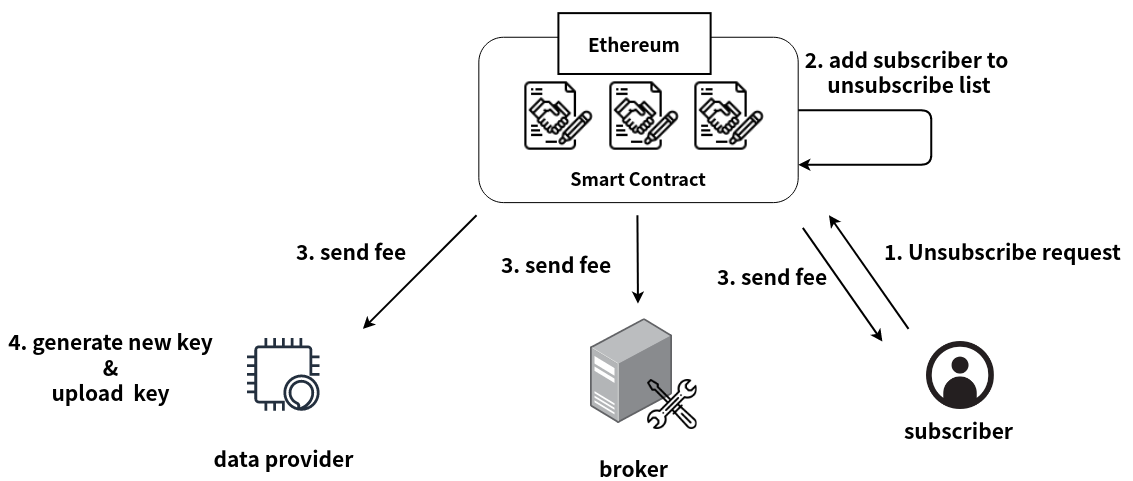
\includegraphics[width=3.5in]{unsubscribe}
    \caption{Once a data consumer launch a unsubscription procedure, he/she is added to unsubscriber list and the Product Contract will distribute the funds to provider, broker and consumers respectively. Then, the data provider will generate a new encryption key and upload it for every remaining subscribers.}
    \label{fig:unsubscribe}
\end{figure}

\subsection{Launch a Refund}
\label{section:refund}
Data subscription is a high risk in which data provider may not upload data as the agreement set after receiving the subscription fee. Therefore, in our proposed architecture, data consumers can trigger a refund procedure by sending a transaction on Ethereum if the data is not available or defective. When the refund procedure is launched, all consumers vote to decide whether the refund is established. See Fig.~\ref{fig:refund}. Once the ratio of consent votes of refunding is higher than a threshold, the subscription fee is proportionally transferred to the data provider, broker and every consumer as following, where $N$ is the number of consumers in this contract:

\begin{equation}
    F_{DataProvider}(i) = Nprice \frac{i-1}{M} (1-F_{b}) -F_{t}
\end{equation}

\begin{equation}
    F_{Broker}(i) = Nprice \frac{i-1}{M} F_{b} -F_{t}
\end{equation}

\begin{equation}
    F_{Consumer}(i) = price (1-\frac{i-1}{M}) -F_{t}
\end{equation}

\begin{figure}[h]
    \centering
    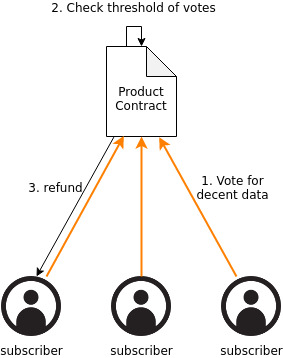
\includegraphics[width=1.5in]{refund}
    \caption{Once a data consumer launch a refund vote, all consumers start voting to decide whether they want a refund. Finally, the establishment of refund is determined by Product Contract after checking the number of votes is larger than a threshold or not.}
    \label{fig:refund}
\end{figure}

However, refund conditions are complicated in the subscription services in the real world, participants can launch a refund in following conditions: First, as proposed methods above, consumers launch a refund vote when the data provider does not upload data as expected after receiving the subscription fee. Nevertheless, multiple issues still need to be investigated such as, consumers can only initiate a refund after getting the data or in a certain time period, the broker should host and set a vote timeline to count the votes, and handling the condition that not enough consumers join the vote need to be considered carefully. Second, brokers operate the subscription platform by earning brokerage fee, which is a deal between brokers and providers. If they can not reach a consensus of the brokerage fee during the subscription period, brokers can launch a refund and refuse to handle the product. Third, the refund could launch by providers when they fail to maintain products as committed.

\section{Evaluations}
\label{section:evaluation}
We evaluate the cost of operating the subscription-based data trading infrastructure in two aspects: 1) Evaluate the cost of adopting MAM on devices, since it is the most commonly used component to data provider. 2) Evaluate the minimum cost for participants to sustain or subscribe to a data product via Product Contract.

\subsection{MAM Performance Evaluation}
\label{section:mam_performance}
It is worth making a claim that all participants in the data subscription platform do not need to hold an IOTA full node which maintains the transaction history and exchanges information of the Tangle. Each role is only required to run client libraries and communicate with IOTA full nodes to interact with the Tangle. Therefore, in the following evaluations, all devices run with client library only.

MAM is a secure and validatable data storage of the proposed architecture. And publishing data to MAM is the primary key to resolve all the difficulties discussed in previous sections. The interactions between data providers and MAM can be frequent. Data providers can either upload data in a short time interval or maintain multiple MAM channels or endpoints at the same time, hence the operation of MAM is one of the potential bottlenecks in the data subscription platform.

In this section, time measurement is evaluated in two MAM operations: channel/endpoint creation and data attachment to endpoints. To perform the evaluation assessment, a personal computer (PC, 3.2GHz 64-bit 6-core i7-8700 with 16GB DDR4 RAM) and a Raspberry Pi 3 Model B (1.2 GHz 64-bit quad-core ARM Cortex-A53 with 1GB LPDDR2 RAM) have been used to run MAM.

\subsubsection{Channel / Endpoint Creation}
The length of a channel or endpoint is $2^{height}-1$ where \textit{height} is the height of Merkle Hash Tree in a Merkle signature scheme (MSS), and the "$-1$" is for announcing the ID of next channel or endpoint. A channel with height $n$ can create $2^n-1$ endpoints, and an endpoint with height $m$ can attach $2^m-1$ messages, therefore the capacity of a channel is $2^{nm}-2^n-2^m+1$ messages in total. The greater the \textit{height} of MSS, the longer the channel/endpoint, however the higher the computational power required. In this task, both channel and endpoint creation are tested and the \textit{height} is set from 1 to 7 which is quite enough for data providers to upload data. The results are shown in Table \ref{tab:channel_create} and Table \ref{tab:endpoint_create}. The time duration for each \textit{height} is the average time of running 100 rounds.

\begin{table}[htbp]
    \caption{Time measurement of channel creation}
    \label{tab:channel_create}
    \begin{center}
    \begin{tabular}{|c|c|c|}
    \hline
        \textbf{height of MSS} & \textbf{PC (sec)} & \textbf{Raspberry Pi 3 (sec)} \\
        \hline
        1 & 0.26183 & 2.908702 \\
        2 & 0.524076 & 5.805524 \\
        3 & 1.045942 & 11.555660 \\
        4 & 2.092989 & 23.178036 \\
        5 & 4.19515 & 46.164079\\
        6 & 8.361586 & 92.320173\\
        7 & 16.651607 & 185.292243\\
        \hline
    \end{tabular}
    \end{center}
\end{table}

\begin{table}[htbp]
    \caption{Time measurement of endpoint creation}
    \label{tab:endpoint_create}
    \begin{center}
    \begin{tabular}{|c|c|c|}
    \hline
        \textbf{height of MSS} & \textbf{PC (sec)} & \textbf{Raspberry Pi 3 (sec)} \\
        \hline
        1 & 0.256425 & 2.887064 \\
        2 & 0.505679 & 5.767912 \\
        3 & 0.999524 & 11.550455 \\
        4 & 1.994017 & 23.260508 \\
        5 & 3.965007 & 46.748366 \\
        6 & 7.918925 & 93.182975 \\
        7 & 16.561419 & 186.064562 \\
        \hline
    \end{tabular}
    \end{center}
\end{table}

The results of Table \ref{tab:channel_create} and Table \ref{tab:endpoint_create} are plotted in Fig.~\ref{fig:mam_create}. Since the creation of channel and endpoint are MSS calculations, the curves of the same hardware are nearly identical. On the other hand, the performance of Raspberry Pi 3 is acceptable when \textit{height} is smaller than 4, but time grows rapidly when \textit{height} is 5 or above. And the performance of PC remains acceptable even \textit{height} gets to 7. The results indicate that MAM channel/endpoint creation is a laborious job for a Raspberry Pi 3 when data providers need a longer channel/endpoint, which is one of the reason that MAM operations should be forwarded to brokers.
 
\begin{figure}[!t]
    \centering
    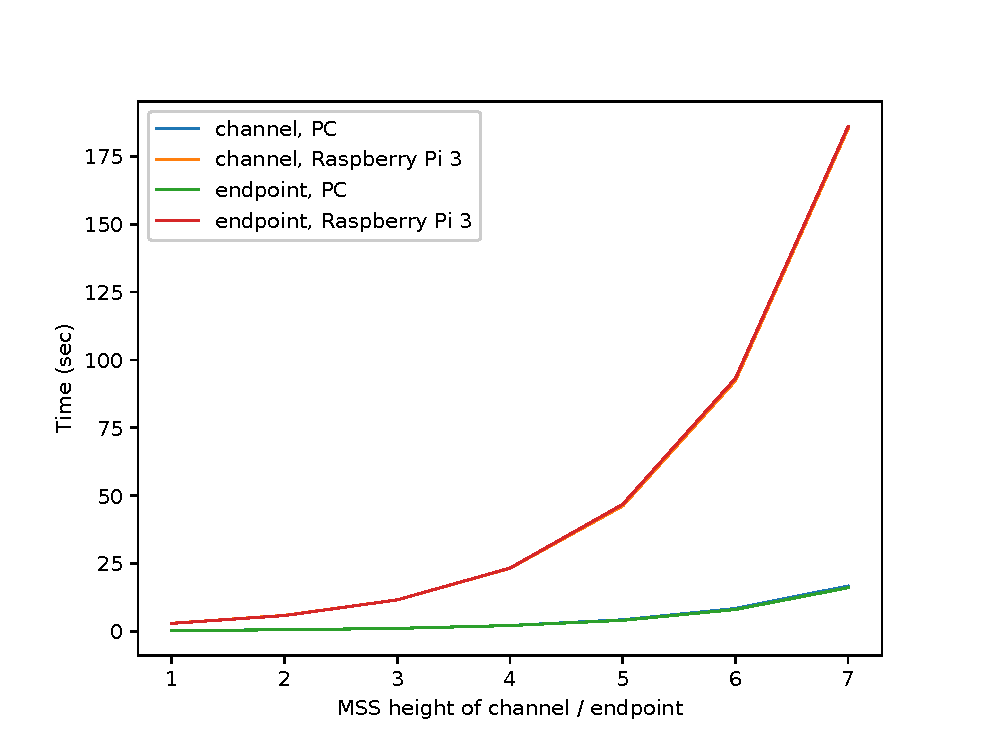
\includegraphics[width=3.in]{mam_create}
    \caption{Time cost of MAM creation.}
    \label{fig:mam_create}
\end{figure}

\subsubsection{Messages Publishment}
Publishing a message to MAM is attaching a zero-value transaction to the Tangle which requires two processes:
\begin{itemize}
    \item    Tips selection: In the IOTA protocol, a new-coming transaction needs to pick up 2 existed transactions called tips to reference and verify. The tips are provided by IOTA full nodes.
    \item    Proof-of-Work (PoW): An algorithm that prevents Denial of Service and spam attacks on a network. A computationally hard puzzle to solve, but easy to verify.
\end{itemize}

Tips selection requires a stable network connection to wait for the response from IOTA full nodes, and PoW requires enough computation resources to perform. Fig.~\ref{fig:mam_send} shows the probability distribution function of publishing a message to MAM endpoint. The time of Raspberry Pi 3 distributed widely since the randomness of PoW has a huge impact while all the tests on PC remain in an acceptable range.

\begin{figure}[!t]
    \centering
    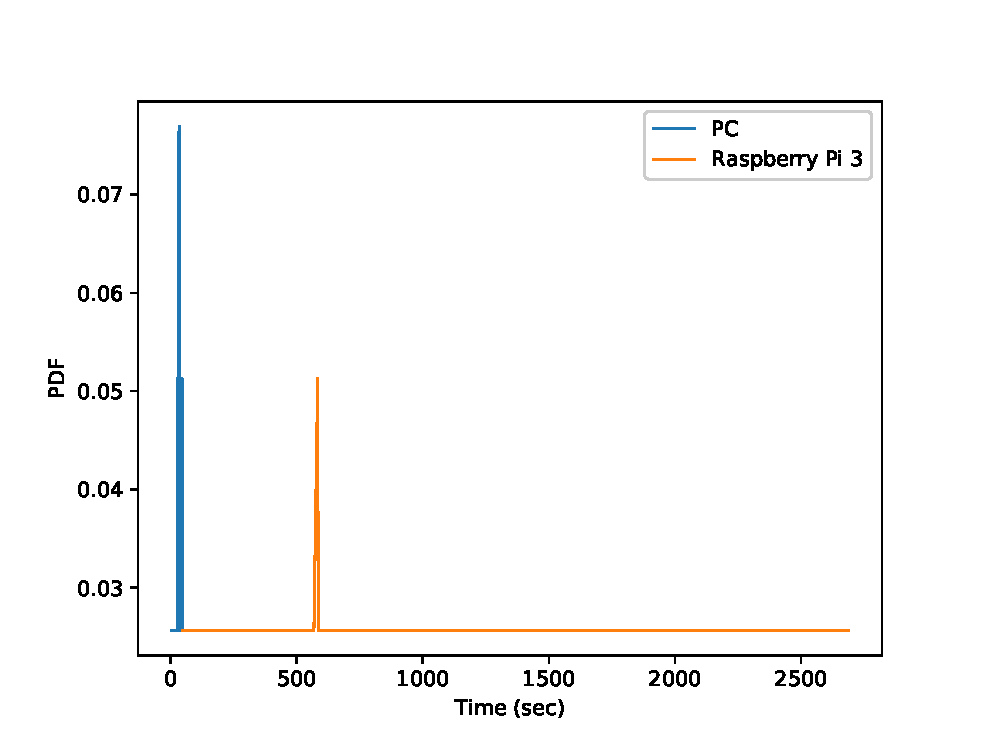
\includegraphics[width=3.in]{mam_send}
    \caption{The probability distributed function of time cost for sending a message through MAM.}
    \label{fig:mam_send}
\end{figure}

The simulation results above indicate that MAM is difficult for low-level sensor devices to run, whereas these kind of devices are the majority of hardware in the IoT scenarios. Furthermore, sensors with low computing power and unstable internet connection are not able to have enough resources to handle data collection, data transmission on MAM, and even trading process with subscribers simultaneously.

Therefore, transferring MAM operations to brokers while ensuring the profit and privacy of providers through blind signatures can effectively solve performance problems and lower the threshold to participate in such a framework. Brokers can be PCs or powerful machines that run Ethereum client and Tangle-accelerator, where Ethereum client is used to interact with Ethereum and Tangle-accelerator provides PoW acceleration and MAM delegation. Fig.~\ref{fig:rpi3_pow} shows the time cost of sending a MAM message with local Pow on Raspberry Pi 3 and remote Pow on Tangle-accelerator. However, MAM operations still cost a considerable time that improving the performance of MAM is an essential issue that needs to be done for the next step.

\begin{figure}[!t]
    \centering
    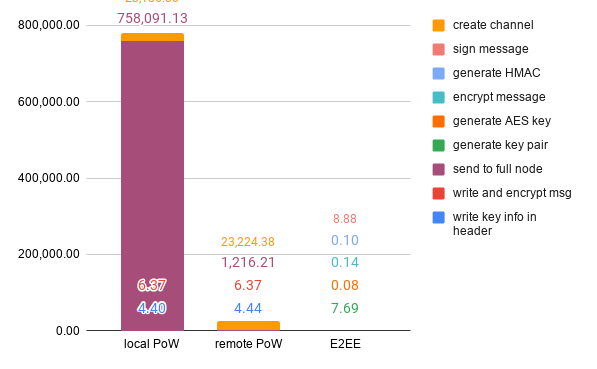
\includegraphics[width=3.5in]{rpi3_pow}
    \caption{Local PoW vs. Remote PoW}
    \label{fig:rpi3_pow}
\end{figure}

\subsection{MAM vs. the delegated MAM}
\label{section:smart_contract_evaluation}

\subsubsection{Experiment}
Applying remote PoW greatly reduces the elapsed time. Channel creation is the next primary barrier for low-level devices to broadcast MAM message. With employing delegated MAM and E2EE, MAM channel creation would be delegated by tangle-accelerator which dramatically enhances the efficiency and makes MAM available for low-level devices. What follows is the performance comparison between MAM and delegated MAM (E2EE) for different payload sizes. Elapsed time for internet communication and PoW are not included, because the following processes starting from sending messages to tangle-accelerator are the common steps. Excluding the common steps allows us to compare the performance between MAM and delegated MAM more clearly. In addition, MAM Channel creation and E2EE asymmetric key pair generation are not included, too. The two excluded steps take much more time than encrypting messages only, so counting these two steps would cause extreme values. In the E2EE protocol framework, we choose SHA-256 for HMAC, AES-CBC for symmetric encryption, and Curve P-256 for ECDSA, respectively.

The steps counted in MAM benchmark including:
\begin{itemize}
    \item Encrypt input payload
    \item Publish final message on IOTA Tangle
\end{itemize}

The steps counted in E2EE benchmark including:
\begin{itemize}
    \item Generate symmetric key for encryption
    \item Hash input payload
    \item Encrypt input payload
    \item Transmit final message to tangle-accelerator
\end{itemize}

\begin{table}[htbp]
    \caption{Compare the performance between MAM and E2EE on Raspberry Pi}
    \label{tab:mam_vs_e2ee}
		\centering
        \begin{tabular}{|c||c|c|}
        \hline
            \textbf{size (bytes)} & \textbf{MAM(ms)} & \textbf{E2EE(ms)} \\
            \hline
            100 & 20.28 & 9.21 \\
            500 &  26.92 & 9.27 \\
            900 & 32.02 &  9.35  \\
            1300 & 36.67 & 9.41 \\
            1700 & 40.55 & 9.54 \\
            \hline
        \end{tabular}
\end{table}

It the Table~\ref{tab:mam_vs_e2ee}, a comparison of the two result reveals elapsing time of E2EE is obviously less than elapsing time of MAM which shows the E2EE process presented in the paper is a much more appropriate solution for resource-constrained systems to send authenticated streaming data.

\begin{equation}
    \label{eq:lin_mam}
    y=0.0126 x+19.979  
\end{equation}

\begin{equation}
    \label{eq:lin_e2ee}
    y=0.0002 x+9.174
\end{equation}

The Eq.~\ref{eq:lin_mam} and Eq.~\ref{eq:lin_e2ee} are the linear equation for the experiment data of MAM and E2EE respectively. Apparently, the slope of the result of MAM is much greater than the result of E2EE. The small slope of E2EE ensures E2EE can consistently perform in an acceptable time range.

\subsubsection{Time Complexity}
With the given E2EE protocol framework, ECDSA would take constant time under our situation, since the string needed to be signed is in fixed length. HMAC and AES-CBC are the procedures that cost most of the elapsed time. Time complexity of HMAC with SHA-256 is $O(n)$.\cite{hmac_time_complexity} Block cipher takes constant time for a single block which causes the time complexity is $O(n)$, too. Therefore, the E2EE protocol framework takes only linear time versus arbitrary string length. Applying mature cryptographic functions (e.g. SHA-256, AES-CBC, etc), ensures gentle slope as Eq.~\ref{eq:lin_e2ee} shows.

\subsection{Smart Contract}
In this experiment, we investigate the cost of executing Product Contract with Ethereum web browser-based IDE Remix that we can define the minimum cost, which data providers should pay in order to launch a product and processing trade.  On top of this evaluation, data providers can consider how to set the price to eventually generate profits. The estimated cost is in Ether, which is 238 USD at the time of writing, yet the price is dynamic from time to time. To conquer this condition, the authors in \cite{MindMyValue} suggested to analyze with a fixed range of Gas price,  yet the main drawback of low Gas price is the increase of time required before a transaction is validated. According to the report of Ethereum network\cite{ethereumChart} in 2020 (January to June), we set this range from 7.3 Gwei to 26.5 Gwei, which is $7.3 \times 10^{-9}$ and $2.65 \times 10^{-8}$ Ether respectively, the minimum average and average gas price. The Gas usage estimation is shown in Table.~\ref{tab:gas}.

\begin{table}[h]
    \caption{Gas consumption for each function of Product Contract}
    \label{tab:gas}
    \resizebox{0.5\textwidth}{!}{
    \begin{tabular}{|c|c|c|c|}
        \hline
        \textbf{function} & \textbf{sender} & \textbf{Gas used} \\
        \hline
        generate contract & broker & 2558980 \\
        subscribe product & consumer & 72259 \\
        upload hashed key & provider & 68276  \\
        upload encryption key to consumer & provider & 86614 \\
        upload certified key & broker & 131535 \\
        update amount of uploaded data & broker & 32157 \\
        unsubscribe & consumer & 8234 \\
        request refund & consumer & 12067 \\
        withdraw & broker & 11313 \\
        \hline
    \end{tabular}
    }
\end{table}

Note that data uploading is only related to MAM operations on IOTA, which does not require any fees. Therefore, the Gas estimation only includes trading processes. Creating a Product Contract (Listing \ref{lst:constructor}) costs the most Gas (0.164 - 0.596 Ether), providers should have enough Ethers to launch the product at the start. Functions (Listing \ref{lst:key_exchange} (0.012 - 0.044 Ether) and Listing \ref{lst:key_certification} (0.022 - 0.0834 Ether)) that are related to key certification and key exchange need a lot of gas as well. Storage on blockchain is expensive. For instance, an SSTORE operation may cost 20000 gas when the value is set to non-zero from zero according to Ethereum Yellow Paper\cite{Ethereum}. However, in our trading model, we preserve a lot of information in the Product Contract in order to record as more details as possible during trading procedures, such as ciphertexts,  signatures during key certification and key exchange. Especially, in the key exchange protocol, it takes several steps of communications between brokers, data providers, and data consumers via storing states to Product Contract. Therefore, it is worth to explore the usage of the non-interactive zero-knowledge protocol such as zk-SNARKS(zero-knowledge succinct non-interactive argument of knowledge)\cite{Snark} which can generate proofs off-chain and simplify the verification process that could not only reduce network and storage cost but also improve the privacy and security of encryption keys. However, using the zero-knowledge protocol is out of the scope of this paper.

Base on Gas estimation in Table.~\ref{tab:gas}, we calculate the exact Ether with Formula~\ref{equa:ether_calculation} that data providers and data consumers need during the trade in Table.~\ref{tab:ether}. We combine the Gas usage of providers and brokers since the brokerage fee is also a critical cost to sustain the trade, which providers should considered. We conclude the three situations during the trading process: 1.) basic cost of a trade, including product launching, subscribing, encryption key uploading and withdraw. 2.) refund operation, the fees needed for launching refund. 3.) unsubscribe operation, the fees needed for launching unsubscription.

\begin{equation}
\label{equa:ether_calculation}
Ethers = Gas \ Price \times Gas \ Amount
\end{equation}

When a consumer request a refund, he/she need to pay 0.0008 - 0.0003 Ether additionally. Then if the refund established, all participants will withdraw the payment, which is already included in the basic cost. Observing the situation of unsubscribe operation, it does not cost much Ether for consumers. However, the data provider needs to update all encryption keys for remaining consumers that \textit{update encrypt key} will be triggered $N$ times, where $N$ is the number of remaining subscribers. This would cost data providers a lot if the unsubscription is frequent or many remaining consumers are left. Hence, an efficient, low-cost, and secure way to perform access control while recording the unsubscription process transparent is important. An alternative strategy coming up with the latest development of MAM, which is renaming to Streams\cite{stream}, provides new functionality for subscribers to unsubscribe to data streams, thus, it is possible to perform access control directly through it rather than uploading new encryption key to the Product Contract. Nevertheless, Streams is still in an alpha version, the details and protocol still need to be well studied.

\begin{table*}[h]
    \caption{Data Price Estimation}
    \label{tab:ether}
    \centering
    \resizebox{0.8\textwidth}{!}{
    \begin{tabular}{|c|c|c|c|c|c|}
        \hline
        \textbf{condition} & \textbf{sender} & \textbf{\makecell{minimum price \\ (Ether)}} & \textbf{\makecell{minimum price \\ (USD)}} & \textbf{\makecell{maximum price \\ (Ether)}} & \textbf{\makecell{maximum price \\ (USD)}} \\
        \hline
        \multirow{2}{*}{basic cost} & provider & 0.021 & 5.038 & 0.076 & 18.291 \\
         & consumer & 0.00061 & 0.145 & 0.0022 & 0.527\\
        \hhline{|=|=|=|=|=|=|}
        \multirow{2}{*}{refund} & provider & 0 & 0 & 0 & 0 \\
         & consumer & 0.00008 & 0.0209 & 0.0003 & 0.0761 \\
        \hline
        \multirow{2}{*}{unsubscribe} & provider & 0.002N & 0.497N & 0.007N & 1.806N \\
         & consumer & 0.00006 & 0.0143 & 0.0002 & 0.0519 \\
        \hline
    \end{tabular}
    }
\end{table*}

\section{Conclusion}
\label{section:conclusion}
By combining the established standards and openly-developed specifications, this paper proposed a highly decentralized, autonomous publish/subscribe model design that combines data storage and trading together in order to ensure the digital rights of both data providers and consumers during the dynamic data streaming trading. It was built with blockchain network, immutable audit trails, and contracts with an integrated decentralized identity system, to enable the data stream trading by shifting risks from centralized services, ensure the authenticity of all participants, clarify the data ownership, enable secure communication and flexible trading mechanisms.

Compared to previous works, we 1.) identify a trustless data trading infrastructure, 2.) ensure the confidentiality of scalable IoT-based sensor data, and 3.) consolidate the economic incentives in the entire ecosystem. Meanwhile, we consider the heavy workload of the low-level sensors, conduct an experiment which authenticates the data providers to delegate the MAM operations to Tangle-accelerators, and conclude that the performance of the E2EE approach is more fitting than the MAM solution. In particular, this work discusses the workflow for subscription-based IoT data trading: Launching, subscribing, unsubscribing, and refund.

\section{Future Work}
\label{section:future_work}
In the subscription-based data trading, there are some issues worth discussing and improving. Firstly, reduce the Gas usage of trading models, as we mentioned in Section~\ref{section:smart_contract_evaluation}, the key exchange process consumes a lot of Gas due to the frequent store operation. Therefore, it is worth discussing how zero-knowledge protocol could used to exchange the key with lower cost, and even validate the key within transfers. Second, brokers are the key to operating a stable system, since they are irreplaceable either from the view of architecture design or trading procedures. However, issues such as the minimum number of brokers needed to operate the system, and the evaluation of adopting gossip protocol among brokers to gossipped trading status, which enables other brokers to handle trading processes when on crashed.

Third, to let consumers search and find interesting data products, a search engine is needed to collect all distributed data products, which might need the authority to design and run the service. The extending issue of searching is ranking, how would the search service provider rank the products, how would that affect data consumers and providers. Fourth, in our design, we do not restrict the qualifications of data providers and brokers, which is different from operating the App store currently, and it is also an interesting issue to discuss.


\bibliographystyle{IEEEtran}
\bibliography{references}

\end{document}